% based mostly on https://tex.stackexchange.com/questions/6019/drawing-hexagons

\documentclass[border=2mm, tikz]{standalone}
\usetikzlibrary{shapes.geometric}
\begin{document}

%
% x=3*(minimum size)/2
% x=\sqrt{3/4}*(minimum size)/2
%
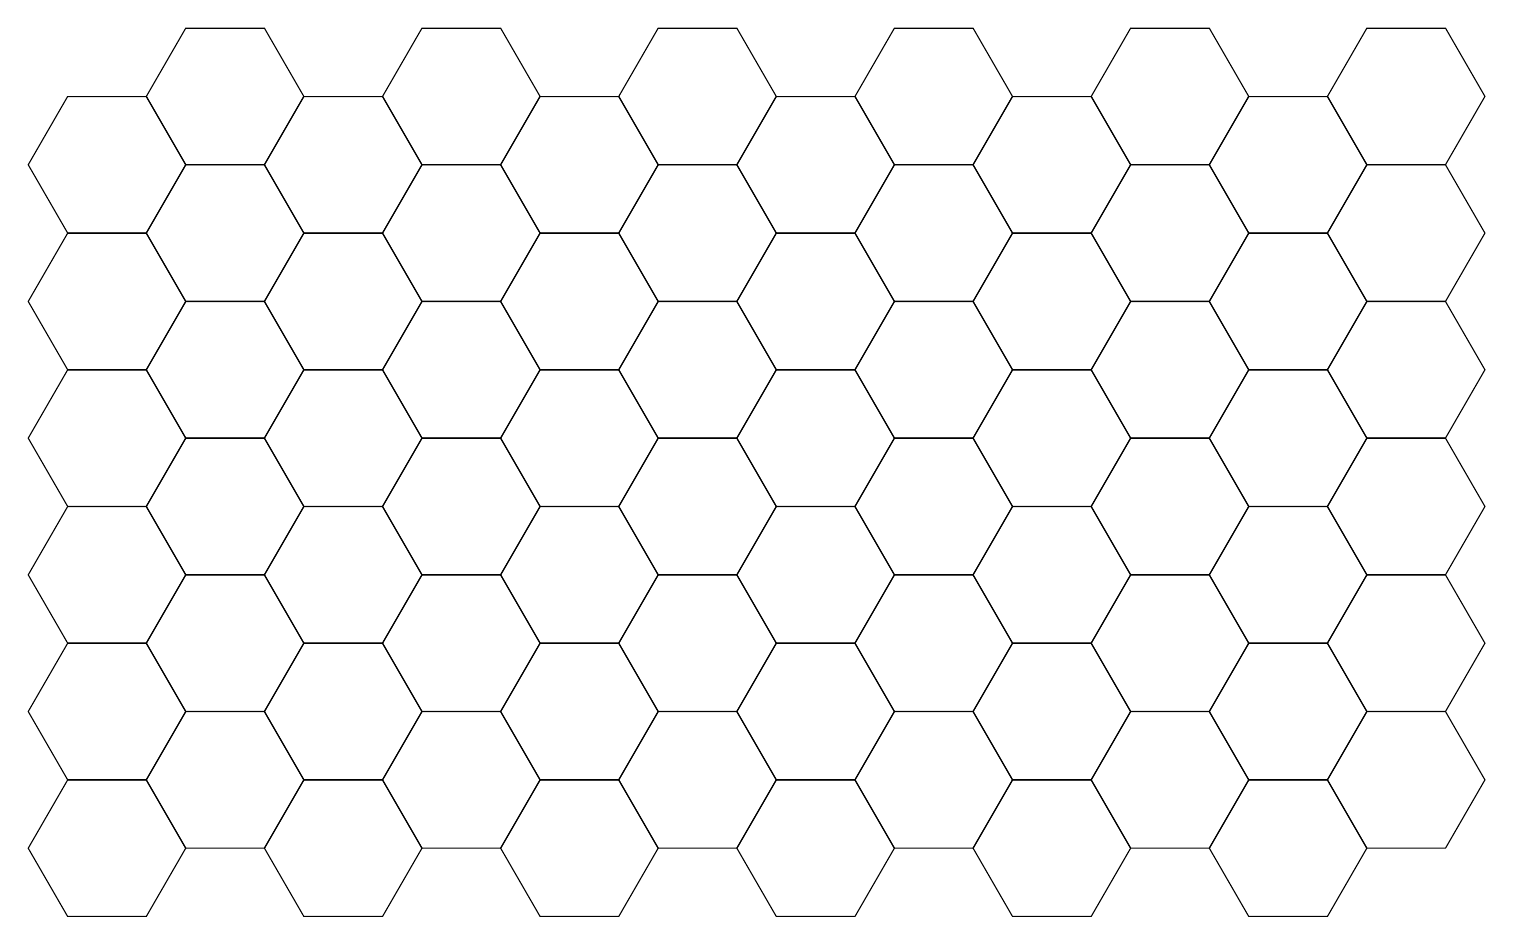
\begin{tikzpicture}[x=15mm,y=8.68mm]
  % some styles
  \tikzset{
    box/.style={
      regular polygon,
      regular polygon sides=6,
      minimum size=20mm,
      inner sep=0mm,
      outer sep=0mm,
      rotate=0,
    draw
    }
  }

\foreach \i in {0,...,5} 
    \foreach \j in {0,...,5} {
            \node[box] at (2*\i,2*\j) {};
            \node[box] at (2*\i+1,2*\j+1) {};
        }

\end{tikzpicture}

\end{document}
